\section{Node Flipping}

The Zhang and Shasha edit distance algorithm is specifically given for ordered trees, that is, the order of child nodes is taken to be significant. In attack trees without sequential conjunction, the order of nodes is not given to be significant~\cite{mauw_foundations_2006,jhawar_attack_2015}. This results in an issue where node


\begin{figure}
    \begin{subfigure}{.45\linewidth}
        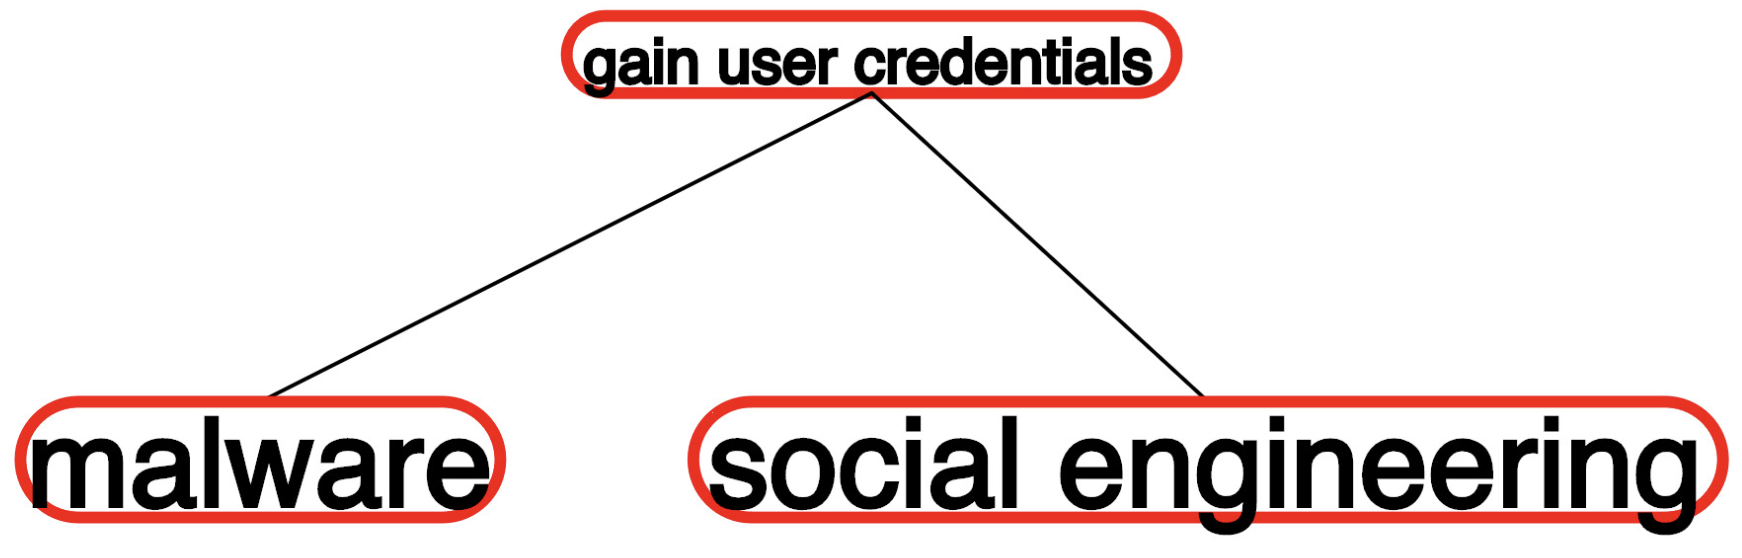
\includegraphics[width=\linewidth]{img/NodeFlip1.png}
    \end{subfigure}
    \begin{subfigure}{.45\linewidth}
        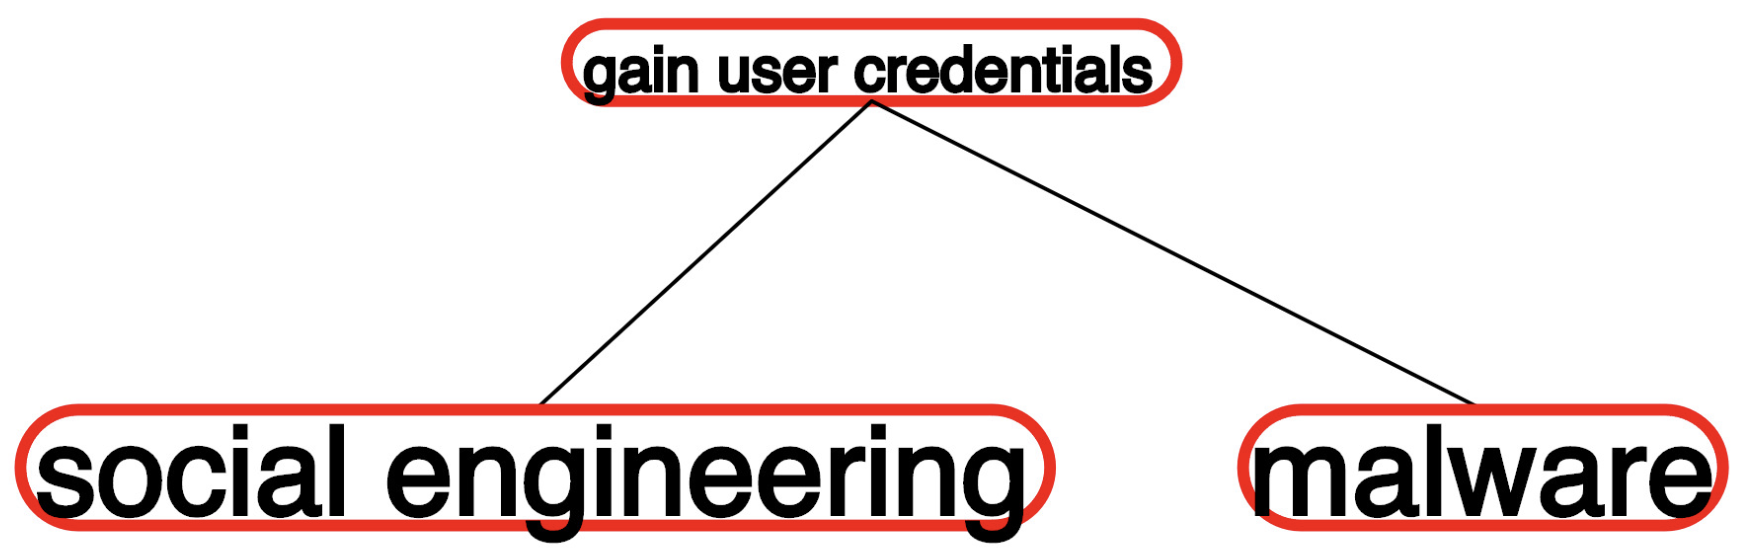
\includegraphics[width=\linewidth]{img/NodeFlip2.png}
    \end{subfigure}
    \caption{Two attack trees (subtrees of the example in Figure~\ref{fig:tartgetAT}) with identical information but different node order. These trees would evaluate to have a distance of 2 (two replacement operations).}
    \label{fig:nodeflipping}
\end{figure}




\subsection{Semantic mapping}

% Prior to calculation, a mapping is made between all nodes with the same labels, and this mapping is used to determine equivalence of nodes within the two trees. The labels of these nodes are typically given to be capital letters of the alphabet. However, in practical application, node labels are typically significantly more complex than mere letters.

% We introduce a new mapping step. As attack trees without sequential conjunction (\SAND\ refinements) are generally given to be unordered, we must implement an unordered semantic mapping. As described by Paa{\ss}en builds upon the work Zhang~\etal\ described for

% The steps:
% \begin{enumerate}
%     \item determine semantic cut off value $\epsilon$
%     \item list all node labels between both trees
%     \item calculate the semantic similarity between all node labels between the two trees
%           \begin{itemize}
%               \item this is given by comparing semantic embeddings
%               \item This is a value between 0 and 1, with 0 being no semantic similarity and 1 being identical semantic similarity
%           \end{itemize}
%     \item starting with node labels with the highest semantic similarity
%     \item remove these labels from both lists
%     \item repeat until at least one list is empty, or all semantic similarity values are below $\epsilon$
% \item Once we have our mappings, we reorder siblings as best as possible
% \begin{enumerate}
%     \item Starting with leaves, siblings can be swapped for no cost
%     \item Done if it improves the mapping
%     \item \textit{may result in local minima issues - but will be optimal enough}
% \end{enumerate}
% \end{enumerate}